\newif\ifsolutions
\solutionstrue % Show solutions
%\solutionsfalse % Hide solutions

\documentclass{article}
\usepackage{geometry}
\geometry{margin=1in}
\usepackage{tikz}
\usepackage{amssymb}

% fleqn allows setting indent of display math
\usepackage[fleqn]{amsmath}
\setlength{\mathindent}{0pt} % Set indent
% Disable equation numbering (https://tex.stackexchange.com/a/360378)
\makeatletter
\renewcommand\tagform@[1]{}
\makeatother

% Allow Unicode (some, e.g., © and £ at least)
% https://tex.stackexchange.com/questions/370278/is-there-any-reason-to-use-inputenc
\usepackage[utf8]{inputenc}

% Hyperlinks
\usepackage{hyperref}
\hypersetup{colorlinks=true, urlcolor=blue, linkcolor=blue}

% Prevent indentation of paragraphs
\setlength\parindent{0pt}
\setlength{\parskip}{\baselineskip}

% Spacing above/below equations
% https://tex.stackexchange.com/a/69678
\AtBeginDocument{%
 \abovedisplayskip=-\parskip
 \abovedisplayshortskip=-\parskip
 \belowdisplayskip=0pt
 \belowdisplayshortskip=0pt
}

% Allow 3 additional subsection levels
% https://tex.stackexchange.com/a/60212
\usepackage{titlesec}
\setcounter{secnumdepth}{6}
% H4 in HTML
\titleformat{\paragraph}{\normalfont\normalsize\bfseries}{\theparagraph}{1em}{}
\titlespacing*{\paragraph}{0pt}{3.25ex plus 1ex minus .2ex}{1.5ex plus .2ex}
% H5 in HTML
\titleformat{\subparagraph}{\normalfont\normalsize\bfseries}{\thesubparagraph}{1em}{}
\titlespacing*{\subparagraph}{0pt}{3.25ex plus 1ex minus .2ex}{1.5ex plus .2ex}
% H6 in HTML
\titleformat{\subsubparagraph}{\normalfont\normalsize\bfseries}{\thesubsubparagraph}{1em}{}
\titlespacing*{\subsubparagraph}{0pt}{3.25ex plus 1ex minus .2ex}{1.5ex plus .2ex}

% So enumerate at all levels is numbers
% https://tex.stackexchange.com/questions/78842/nested-enumeration-numbering
\renewcommand{\labelenumii}{\arabic{enumii}.}
\renewcommand{\labelenumiii}{\arabic{enumiii}.}
\renewcommand{\labelenumiv}{\arabic{enumiv}.}

\renewcommand{\mbox}{\text}
\newcommand{\ds}[0]{\displaystyle}
\newcommand{\ihat}[0]{\hat{\boldsymbol{\imath}}}
\newcommand{\jhat}[0]{\hat{\boldsymbol{\jmath}}}
\newcommand{\khat}[0]{\hat{\boldsymbol{k}}}
\newcommand{\xhat}[0]{\hat{\mathbf{x}}}
\newcommand{\yhat}[0]{\hat{\mathbf{y}}}
\newcommand{\zhat}[0]{\hat{\mathbf{z}}}
\newcommand{\rhat}[0]{\hat{\mathbf{r}}}
\newcommand{\bfvec}[1]{\vec{\mathbf{#1}}}
\newcommand{\bfcdot}[0]{\boldsymbol{\cdot}}

\usepackage{fancyhdr}
\pagestyle{fancy}
\lhead{Lenz's Law}
\rhead{\thepage}
\fancyfoot{}

\begin{document}

\section{Introduction}

\subsection{Magnetic Flux}

A changing magnetic flux through a closed conducting loop \emph{induces} the flow of a current in the loop.

In this activity, we will deal with a conducting loop that has a current that is not driven by a battery -- it will be driven by a change in magnetic flux through the loop. This change will \emph{induce} a current, and this induced current will create what we will refer to as an \emph{induced} magnetic field.

The general equation for magnetic flux is:

$$
\Phi_B = \int \bfvec{B}\cdot d\bfvec{A}
$$

If the magnitude of the magnetic field is not changing and the angle between the magnetic field vector and the area vector does not change, then integration is not required, and we can write

$
\Phi_B = \bfvec{B}\bfcdot \bfvec{A}
$
or, equivalently, $\Phi_B = BA\cos\phi$, where $\phi$ is the angle between the area vector, $\bfvec{A}$, and $\bfvec{B}$.

There are three ways in which $\Phi_B$ can change:

\begin{enumerate}

  \item The magnitude of $\bfvec{B}$ (that is, $B$) can change. To do this, a magnet can be moved closer or farther away from a loop, a loop can be moved closer or farther away from a magnet, or the current that is generating the magnetic field can be changed. See Example 29.1 in the textbook for an example of the creation of a changing magnetic field with an electromagnet.

  \item The area $A$ can change. To do this, the loop cross--section can be expanded or contracted by heating or cooling a wire or, more commonly, using a device called a slidewire generator (see Example 29.5 in the textbook).

  \item The angle $\phi$ can change. To do this, a conducting loop can be rotated (see Example 29.3 in the textbook). Electric motors use changes in $\phi$ to convert mechanical energy to electrical energy.

\end{enumerate}

In this activity, you will determine the direction of the induced current in a conducting loop due to a changing magnetic flux through its area using Lenz's law for cases 1. and 2.

%Although Lenz's law can be used for case 3., we generally use Faraday's law first and then ask if our answer is consistent with Lenz's law. This is covered in a separate activity. Additionally, Lenz's law can be used to determine the direction of force or torque required by an external agent to cause the change in flux through the loop. This is also covered in a separate activity.

\newpage

\subsection{Lenz's Law}

As described in the textbook,

{\bf Lenz's Law:} The direction of any magnetic induction effect is such as to oppose the cause of the effect.

Here, we'll use a longer but more descriptive definition.

{\bf Lenz's Law alternative}: When the magnetic flux due to an external source of a magnetic field through a conducting loop changes, a current appears (is induced) in the loop. The induced current creates an induced magnetic field. The direction of the induced current is such that the induced magnetic field opposes the change in flux.

In the examples given, we will first find the direction of the induced magnetic field needed to oppose a change in flux due to an external source of a magnetic field. Then, we will ask what direction of the induced current is consistent with this induced magnetic field using the current loop right--hand rule, which is described in the next section.

(Lenz's law follows from Faraday's law. In principle, Faraday's law, with careful attention paid to signs, can be used to determine the direction of induced current, in which case Lenz's law is not needed. In a similar way that using the right--hand rules to determine the general direction for force can be used to check your math on a cross--product, Lenz's Law provides a check on the direction of the induced current when using Faraday's law.)

\section{Current Loop Right--Hand Rule}

Given a loop of current in a plane, one can determine the direction of its magnetic field near the center using the current loop right--hand rule: wrap your fingers around the loop in the direction of the current -- your thumb points in the direction of the magnetic field.

\input{figures/Figure-28.12_Young_Freedman_14th_Edition.png}

\textbf{Figure 28.12 of Young and Freedman 14th Edition}

\newpage

\section{$B$ Changing}

\subsection{Example}

A spatially uniform external magnetic field points out of the page, and its magnitude increases over time.

\input{figures/Field_Out_Of_Page.tikz}

\begin{enumerate}

  \item What is the direction of an induced magnetic field in the gray region that opposes the change in the magnetic flux?

  \item What is the direction of induced current in the loop that is consistent with the induced magnetic field found in part 1?

\end{enumerate}

{\bf Answer}:

To determine the direction of the induced magnetic field, we draw field lines through the area at $t=0$ and then a short time later. On the left--hand side of the following figure, field lines are shown pointing out of the page. A short time later, at $t=\Delta t$, $B_{\text{ext}}$ has increased, so we draw more field lines pointing out of the page.

The induced magnetic field is in the direction that opposes the change in magnetic flux, so the induced field must be in to the page. (The induced magnetic flux will not exactly cancel the increase in flux; the magnitude of the induced magnetic flux will depend on how much current is induced, which depends on the resistance of the wires.)

Finally, we ask what direction of induced current is consistent with a $B_{\text{ind}}$ directed into the page. Using the current loop right--hand rule, it is a clockwise current.

\input{figures/Field_Out_Of_Page_B_Increasing.tikz}

\newpage

\subsection{Problems}

\subsubsection{}

A spatially uniform external magnetic field points into the page, and its magnitude increases over time.

\input{figures/Field_In_To_Page.tikz}

\begin{enumerate}

  \item Draw representitive field lines at $t=0$ and $t=\Delta t$ as done in the example.

        \ifsolutions

        \else

        \input{figures/Loop_Sketch.tikz}
        \fi

  \item What direction would an induced magnetic field have to be to oppose the change in the magnetic flux?

        \ifsolutions
        {\bf Answer}: Out of the page
        \else

        \fi

  \item What is the direction of induced current in the loop that is consistent with the induced magnetic field found in part 2?

        \ifsolutions
        {\bf Answer}: Counterclockwise
        \else

        \fi

\end{enumerate}

\subsubsection{}

A spatially uniform external magnetic field points into the page, and its magnitude decreases in time.

\input{figures/Field_In_To_Page.tikz}

\begin{enumerate}

  \item Draw representitive field lines at $t=0$ and $t=\Delta t$ as done in the example.

        \ifsolutions

        \else

        \input{figures/Loop_Sketch.tikz}
        \fi

  \item What direction would an induced magnetic field have to be to oppose the change in the magnetic flux?

        \ifsolutions
        {\bf Answer}: Into the page
        \else

        \fi

  \item What is the direction of induced current in the loop that is consistent with the induced magnetic field found in part 2?

        \ifsolutions
        {\bf Answer}: Clockwise
        \else

        \newpage
        \fi

\end{enumerate}

\subsubsection{}

A conducting wire loop is placed in the magnetic field of a solenoid, as shown. Treat the magnetic field of the solenoid as the external magnetic field. Several representative magnetic field lines are shown.

\input{figures/Ring_and_Solenoid.png}

For the following case, determine if an induced magnetic field will appear and, if so, its direction. Then, determine the direction of induced current, if any, in the wire loop.

\begin{enumerate}

  \item The loop is stationary.

        \ifsolutions
        {\bf Answer}: a. No flux change, so no induced magnetic field. b. No current.
        \else
        a. Direction of induced magnetic field:

        b. Direction of current in the loop:
        \fi

  \item The loop is moving to the right.

        \ifsolutions
        {\bf Answer}: As the loop moves to the right, the magnetic field is larger (field lines are more closely spaced). a. To oppose the change in flux, an induced magnetic field pointing to the left is needed. b. The current in the loop is such that the current on the white part of the ring is upwards.
        \else
        a. Direction of induced magnetic field:

        b. Direction of current in loop:
        \fi

  \item The loop is moving to the left.

        \ifsolutions
        {\bf Answer}: As the loop moves to the left, the magnetic field is smaller (field lines are less closely spaced). a. To oppose the change in flux, an induced magnetic field pointing to the right is needed. b. The current in the loop is such that the current on the white part of the ring is downwards.
        \else
        a. Direction of induced magnetic field:

        b. Direction of current in the loop:
        \fi

\end{enumerate}

\subsubsection{}



\tikzset{every picture/.style={line width=0.75pt}} %set default line width to 0.75pt        

\begin{tikzpicture}[x=0.75pt,y=0.75pt,yscale=-1,xscale=1]
%uncomment if require: \path (0,242); %set diagram left start at 0, and has height of 242

%Straight Lines [id:da9391741884541585] 
\draw    (20,110) -- (217,110) ;
\draw [shift={(220,110)}, rotate = 180] [fill={rgb, 255:red, 0; green, 0; blue, 0 }  ][line width=0.08]  [draw opacity=0] (8.93,-4.29) -- (0,0) -- (8.93,4.29) -- cycle    ;
%Straight Lines [id:da5381284642114172] 
\draw    (210,110) -- (390,110) ;
%Shape: Rectangle [id:dp1701563399055186] 
\draw   (60,30) -- (140,30) -- (140,70) -- (60,70) -- cycle ;
%Shape: Rectangle [id:dp04365775921249937] 
\draw   (200,30) -- (270,30) -- (270,70) -- (200,70) -- cycle ;
%Shape: Rectangle [id:dp6674329160586638] 
\draw   (60,150) -- (140,150) -- (140,190) -- (60,190) -- cycle ;
%Shape: Rectangle [id:dp14305010940503493] 
\draw   (200,150) -- (270,150) -- (270,190) -- (200,190) -- cycle ;
%Straight Lines [id:da7178870615335102] 
\draw    (100,70) -- (100,88) ;
\draw [shift={(100,90)}, rotate = 270] [color={rgb, 255:red, 0; green, 0; blue, 0 }  ][line width=0.75]    (10.93,-3.29) .. controls (6.95,-1.4) and (3.31,-0.3) .. (0,0) .. controls (3.31,0.3) and (6.95,1.4) .. (10.93,3.29)   ;
%Straight Lines [id:da9835364258802752] 
\draw    (270,50) -- (288,50) ;
\draw [shift={(290,50)}, rotate = 180] [color={rgb, 255:red, 0; green, 0; blue, 0 }  ][line width=0.75]    (10.93,-3.29) .. controls (6.95,-1.4) and (3.31,-0.3) .. (0,0) .. controls (3.31,0.3) and (6.95,1.4) .. (10.93,3.29)   ;
%Straight Lines [id:da6085880149489133] 
\draw    (140,170) -- (158,170) ;
\draw [shift={(160,170)}, rotate = 180] [color={rgb, 255:red, 0; green, 0; blue, 0 }  ][line width=0.75]    (10.93,-3.29) .. controls (6.95,-1.4) and (3.31,-0.3) .. (0,0) .. controls (3.31,0.3) and (6.95,1.4) .. (10.93,3.29)   ;
%Straight Lines [id:da34065289148350364] 
\draw    (240,190) -- (240,208) ;
\draw [shift={(240,210)}, rotate = 270] [color={rgb, 255:red, 0; green, 0; blue, 0 }  ][line width=0.75]    (10.93,-3.29) .. controls (6.95,-1.4) and (3.31,-0.3) .. (0,0) .. controls (3.31,0.3) and (6.95,1.4) .. (10.93,3.29)   ;

% Text Node
\draw (201,114.4) node [anchor=north west][inner sep=0.75pt]    {$I$};
% Text Node
\draw (88,42.4) node [anchor=north west][inner sep=0.75pt]    {$A$};
% Text Node
\draw (91,162.4) node [anchor=north west][inner sep=0.75pt]    {$C$};
% Text Node
\draw (227,42.4) node [anchor=north west][inner sep=0.75pt]    {$B$};
% Text Node
\draw (228,161.4) node [anchor=north west][inner sep=0.75pt]    {$D$};
% Text Node
\draw (106,78.4) node [anchor=north west][inner sep=0.75pt]    {$v$};
% Text Node
\draw (287,26.4) node [anchor=north west][inner sep=0.75pt]    {$v$};
% Text Node
\draw (151,172.4) node [anchor=north west][inner sep=0.75pt]    {$v$};
% Text Node
\draw (244,205.4) node [anchor=north west][inner sep=0.75pt]    {$v$};


\end{tikzpicture}


In the figure above, there is a current $I$ running through a long straight wire as shown.

For conducting loops A--D that are moving with a velocity in the direction shown, determine if the current flow is zero, clockwise, or counterclockwise. Put your answers on the diagram.

\ifsolutions
{\bf Answer}: The field is out of the page above the long straight wire. Below, it is into the page (See section 28.3 of the Textbook). The magnitude of $\bfvec{B}$ is larger near the wire.

A. Induced field is into page. The current is clockwise.

B. No current.

C. No current.

D. Induced field is out of page. The current is counterclockwise.
\else

\newpage
\fi

\section{$A$ Changing}

\subsection{}

A spatially uniform external magnetic field points out of the page, and it does not change with time. The conducting loop is heated, causing the gray cross--sectional area to increase with time.

\begin{enumerate}

  \item Draw representative field lines at $t=0$ and $t=\Delta t$.

        \ifsolutions

        \else

        \input{figures/Loop_Sketch_Increasing_A.tikz}
        \fi

  \item What direction would an induced magnetic field have to be to oppose the change in the magnetic flux?

        \ifsolutions
        {\bf Answer}: Into the page
        \else

        \fi

  \item What is the direction of induced current in the loop that is consistent with the induced magnetic field found in part 1?

        \ifsolutions
        {\bf Answer}: Clockwise
        \else

        \fi

\end{enumerate}

\subsection{}

An external magnetic field points into the page and it is not changing with time. The conducting loop is cooled causing the gray cross--sectional area to decrease with time.

\begin{enumerate}

  \item Draw representative field lines at $t=0$ and $t=\Delta t$.

        \ifsolutions

        \else

        \input{figures/Loop_Sketch_Decreasing_A.tikz}
        \fi

  \item What direction would an induced magnetic field have to be to oppose the change in the magnetic flux?

        \ifsolutions
        {\bf Answer}: Into the page
        \else

        \fi

  \item What is the direction of induced current in the loop that is consistent with the induced magnetic field found in part 2?

        \ifsolutions
        {\bf Answer}: Clockwise
        \else
        %\newpage
        \fi

\end{enumerate}

\subsection{}

In a region of space where an external magnetic field is spatially uniform, a conducting bar slides along a U-shaped conducting wire (this is known as a ``slidewire generator").



\tikzset{every picture/.style={line width=0.75pt}} %set default line width to 0.75pt        

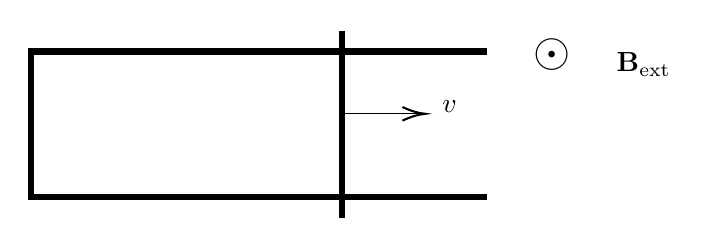
\begin{tikzpicture}[x=0.75pt,y=0.75pt,yscale=-1,xscale=1]
%uncomment if require: \path (0,114); %set diagram left start at 0, and has height of 114

%Shape: Rectangle [id:dp7638554893646261] 
\draw  [line width=2.25]  (20,20) -- (170,20) -- (170,90) -- (20,90) -- cycle ;
%Straight Lines [id:da8020175323566545] 
\draw    (170,50) -- (208,50) ;
\draw [shift={(210,50)}, rotate = 180] [color={rgb, 255:red, 0; green, 0; blue, 0 }  ][line width=0.75]    (10.93,-3.29) .. controls (6.95,-1.4) and (3.31,-0.3) .. (0,0) .. controls (3.31,0.3) and (6.95,1.4) .. (10.93,3.29)   ;
%Straight Lines [id:da966588851849048] 
\draw [line width=2.25]    (170,10) -- (170,100) ;
%Straight Lines [id:da74599236475864] 
\draw [line width=2.25]    (20,20) -- (240,20) ;
%Straight Lines [id:da06687573743311237] 
\draw [line width=2.25]    (20,90) -- (240,90) ;

% Text Node
\draw (261,12.4) node [anchor=north west][inner sep=0.75pt]  [font=\LARGE]  {$\odot $};
% Text Node
\draw (301,19.4) node [anchor=north west][inner sep=0.75pt]    {$\mathbf{B}_{\text{ext}}$};
% Text Node
\draw (217,42.4) node [anchor=north west][inner sep=0.75pt]    {$v$};


\end{tikzpicture}


\begin{enumerate}

  \item What direction would an induced magnetic field have to be to oppose the change in the magnetic flux?

        \ifsolutions
        {\bf Answer}: Into the page.
        \else

        \fi

  \item What is the direction of induced current in the loop that is consistent with the induced magnetic field found in part 1?

        \ifsolutions
        {\bf Answer}: Clockwise.
        \else

        \fi

\end{enumerate}

\end{document}